% Construct a path which minimizes the delay

There's one important observation no matter from which piont we start the visit:

\begin{quote}
\textit{The last visited point must be either at the head or at the end.}
\end{quote}

Suppose this is not the case. Let's denote the last visited point as $p_k$ and the start point as $p_s$. Then $p_k$ lies either in the interval $(p_1, p_s)$ or $(p_s, p_n)$. Because $p_k$ lies within the two intervals, it's impossible to visit $p_1$ and $p_n$ without visiting $p_k$. Thus $p_k$ can't be the last visited point.

Let's consider the \textit{last visited consecutive sequence}. Last visited consecutive sequence is an array of points $A[1..k]$, where:

\begin{enumerate}
\item $A[i]$ and $A[i+1]$ are neighbors on the line
\item $A[i]$ is visited exactly before $A[i+1]$
\item $A[k]$ is the last visited point
\end{enumerate}

According to the observation above, the last visited consecutive consequence is either like $p_k, p_{k-1}, .., p_1$ or like $p_{k+1}, .., p_n$. Suppose the last visited consecutive sequence is at the head, let's visualize what it looks like:\\\\

% Define style for nodes
\tikzstyle{every node}=[circle, draw, fill=black!50,
                        inner sep=0pt, minimum width=4pt]
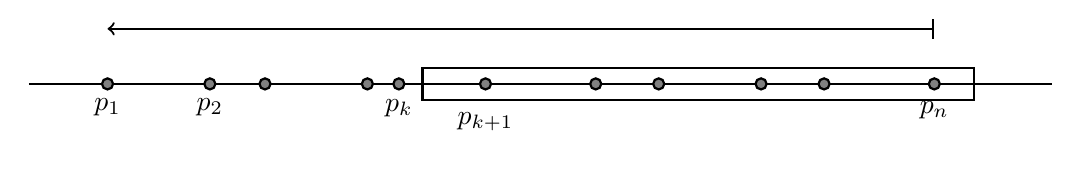
\begin{tikzpicture}[thick]
  \path[draw] (0, 0) -- (13, 0);

  \draw (1, 0) node[label=below:$p_1$] {};
  \draw (2.3,0) node[label=below:$p_2$] {};
  \draw (3, 0) node {};
  \draw (4.3,0) node {};
  \draw (4.7,0) node[label=below:$p_k$] {};

  \draw (5.8, 0) node[label={[label distance=0.3]below:$p_{k+1}$}] {};
  \draw (7.2, 0) node {};
  \draw (8, 0) node {};
  \draw (9.3, 0) node {};
  \draw (10.1, 0) node {};
  \draw (11.5, 0) node[label={[label distance=0.5]below:$p_n$}] {};

  \path[draw] (5, 0.2)-- (5, -0.2) -- (12, -0.2) -- (12, 0.2) -- cycle;

  \draw[->, |->] (11.5, 0.7) -- (1, 0.7);
    
\end{tikzpicture}\quad

In the graph above, $p_k, .., p_2, p_1$ is the last visited consecutive sequence. Then what we can say about the last visited point in $p_{k+1}, .., p_n$? Based on previous observation, we know either $p_{k+1}$ or $p_n$ must be the last visited point. However, if $p_{k+1}$ is the last visited point, we can grow our last visited consecutive sequence $p_k, .., p_2, p_1$ by $p_{k+1}$. Thus, we can conclude:

\begin{quote}
\textit{If $p_k, .., p_2, p_1$ is the last visited consecutive sequence, then the last visited point in $p_{k+1}, .., p_n$ is $p_n$.}
\end{quote}

With the property above, if we are given the optimal solution to the subproblem $p_{k+1}, .., p_n$, then a possible solution to the outer big problem can be constructed by adding the delay of each point in the last visited consecutive sequence. As we know the last visited point in the subproblem is $p_n$, so for each point $p_i$ in the last visited consecutive sequence, its delay is $delay(p_n) + dist(p_i, p_n)$.

Similar arguments hold as well if the \textit{last visited consecutive consequence} is at the end of the array. Then we can decouple the problem into subproblems using following recurrence relation:

\[
OPT(p_1, p_2, .., p_n) = min \left\{
  \begin{array}{ll}
    OPT(p_{k+1}, .., p_n) + \Sigma_{i=1}^{k}(delay(p_n) + dist(p_i, p_n)) & Case 1 \\
    OPT(p_1, p_2, .., p_k) + \Sigma_{i=k+1}^{n}(delay(p_1) + dist(p_i, p_1)) & Case 2 \\
  \end{array}\right.
\]

In \textit{Case 1}, the last visited consecutive sequence is at the head of the array. In \textit{Case 2}, the last visited consecutive sequence is at the end of the array.

The algorithm is straight-forward given the recurrence relation above. The algorithm
calculates the optimal solutions to all possible intervals $p_i, .., p_j$, starting from the base cases
with a single element $p_i$ and finish at $p_1, .., p_n$.

Now let's see the performance of the algorithm. Obviously, there are exactly $n - i + 1$ intervals with a size of $i$. For each interval of size $i$, it has to select one optimal solution among the $2(i-1)$ possible divisions of subprolems. So the total cost is $\Sigma_{i=1}^{n} (n - i + 1) \cdot i = O(n^3)$.